\begin{figure}[htb]
    \begin{center}
        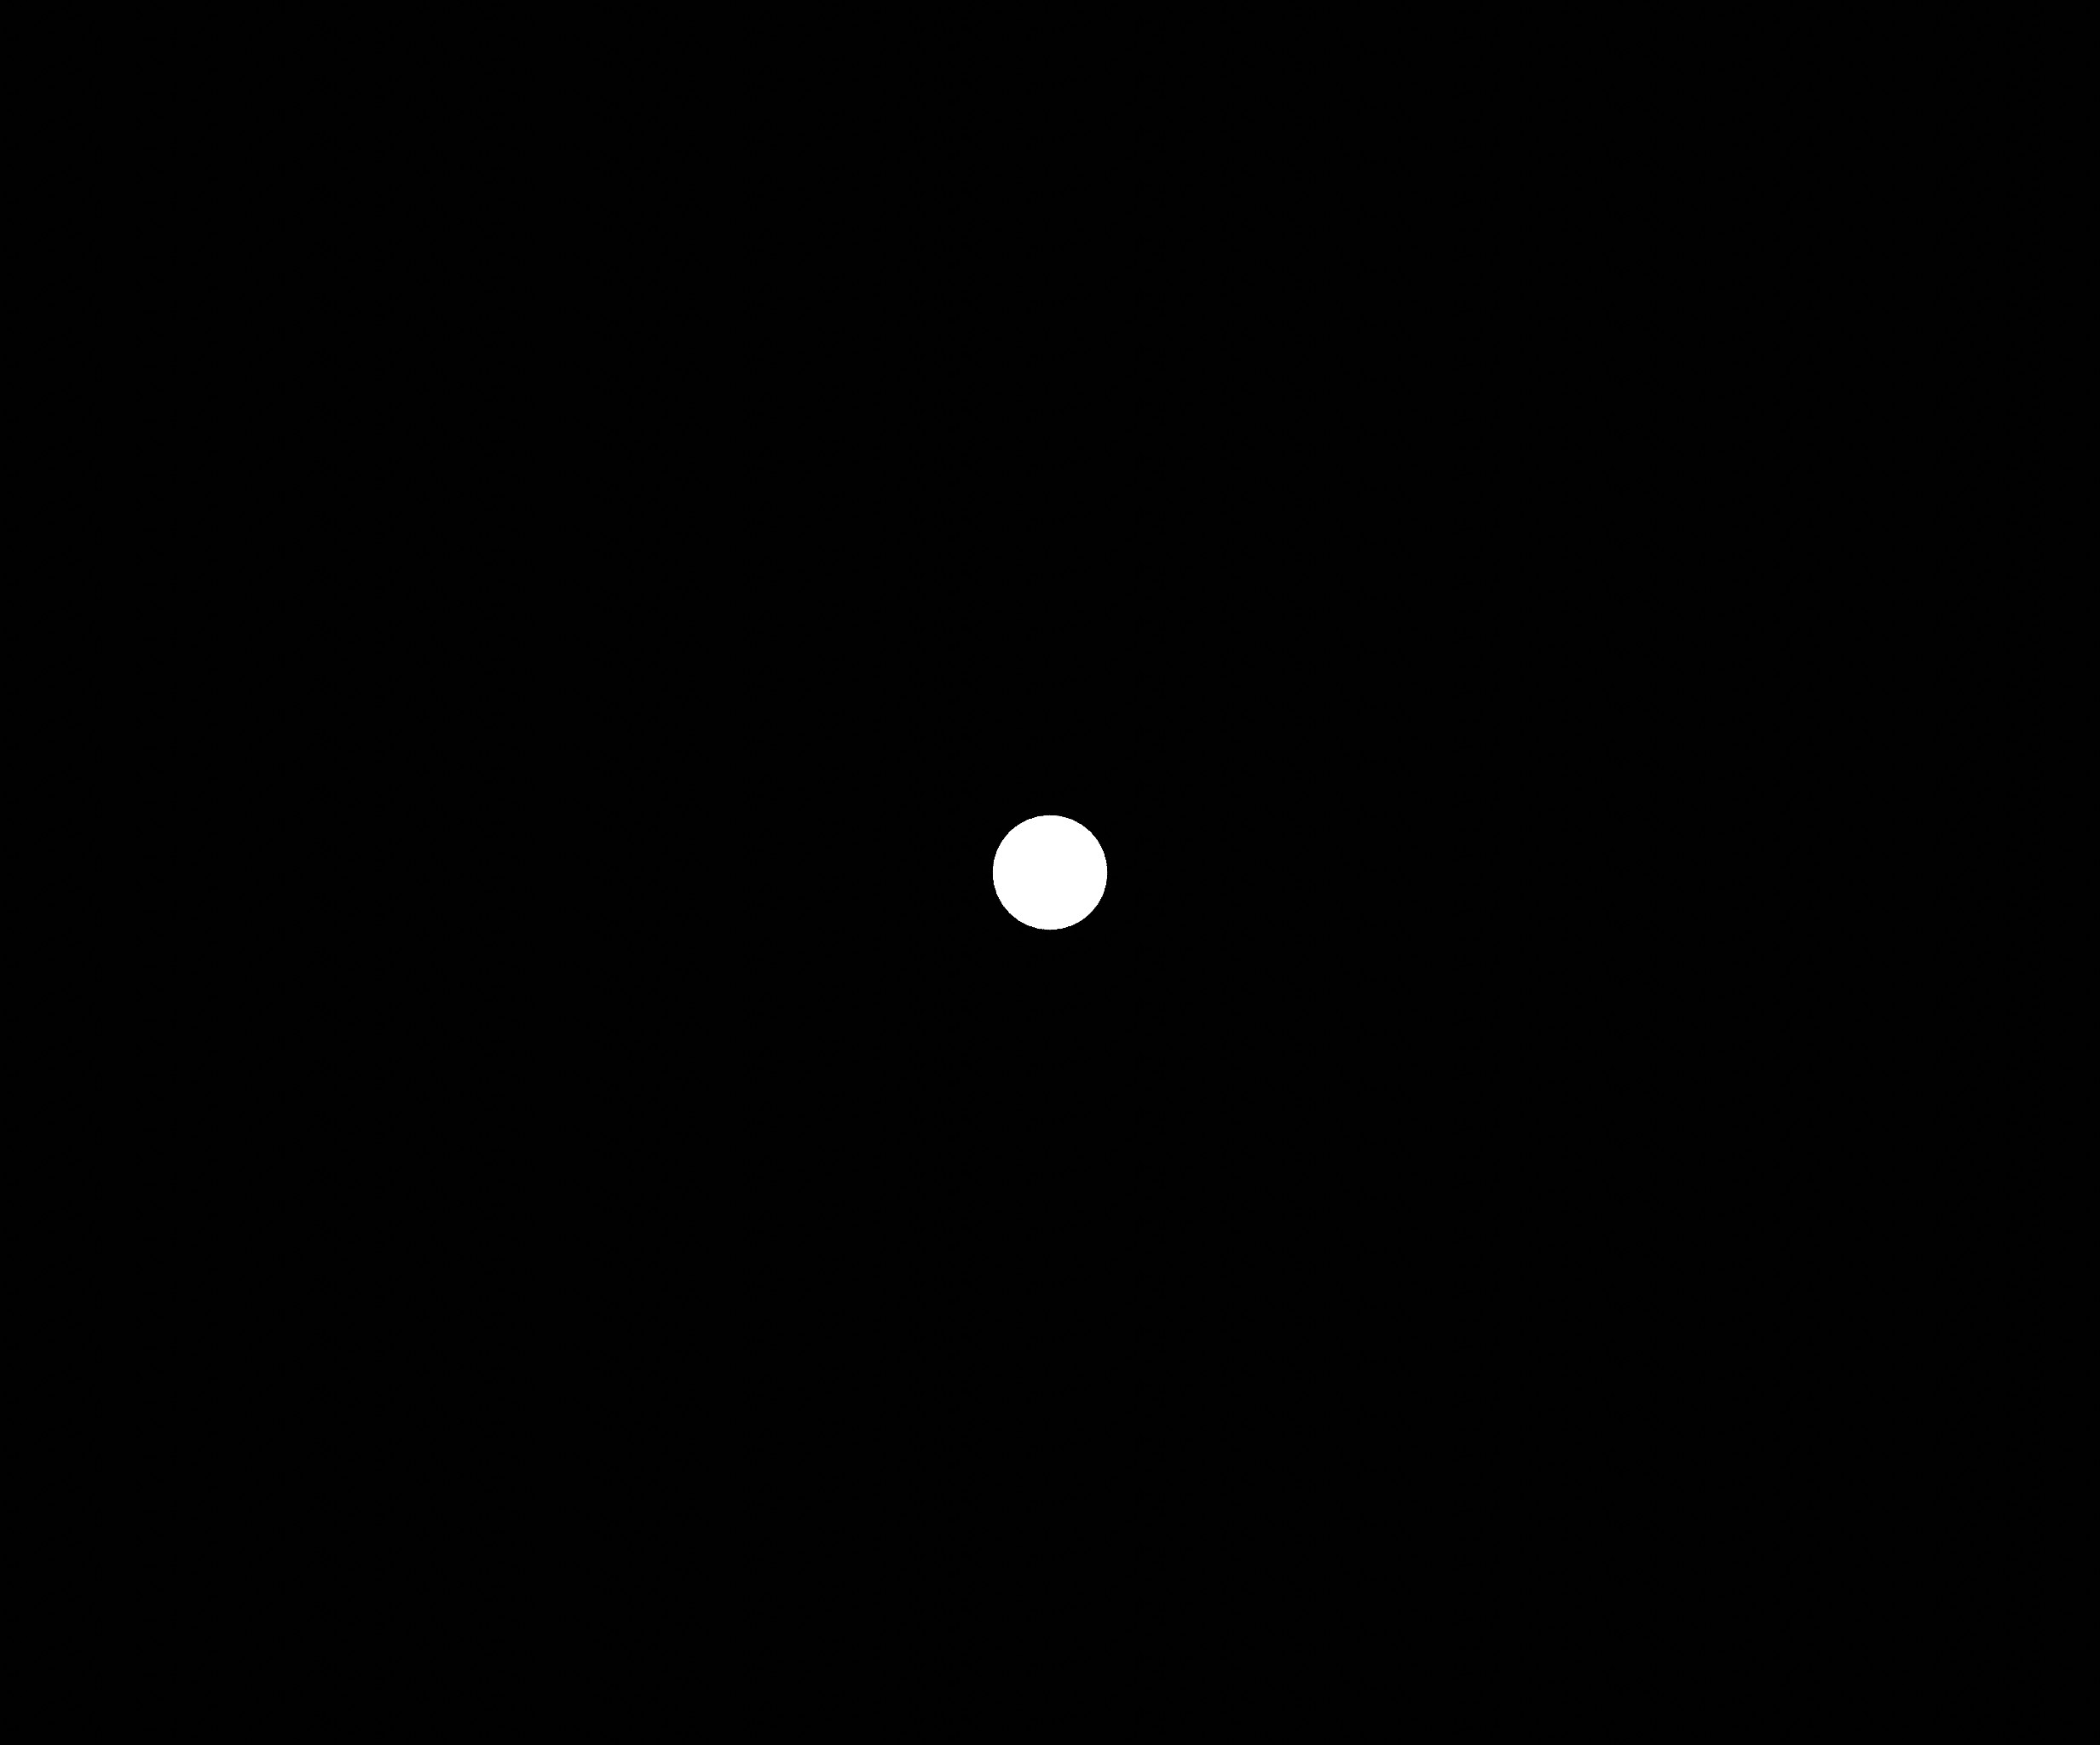
\includegraphics[height=8cm]{doc/thesis/0_figures/cv_skimage/LightRef_2017-08-15T115851-679000.jpg}
    \end{center}
    \caption{LightRef image used in benchmark.}
    \label{fig:bm_light_ref}
\end{figure}

\begin{figure}[htb]
    \begin{center}
        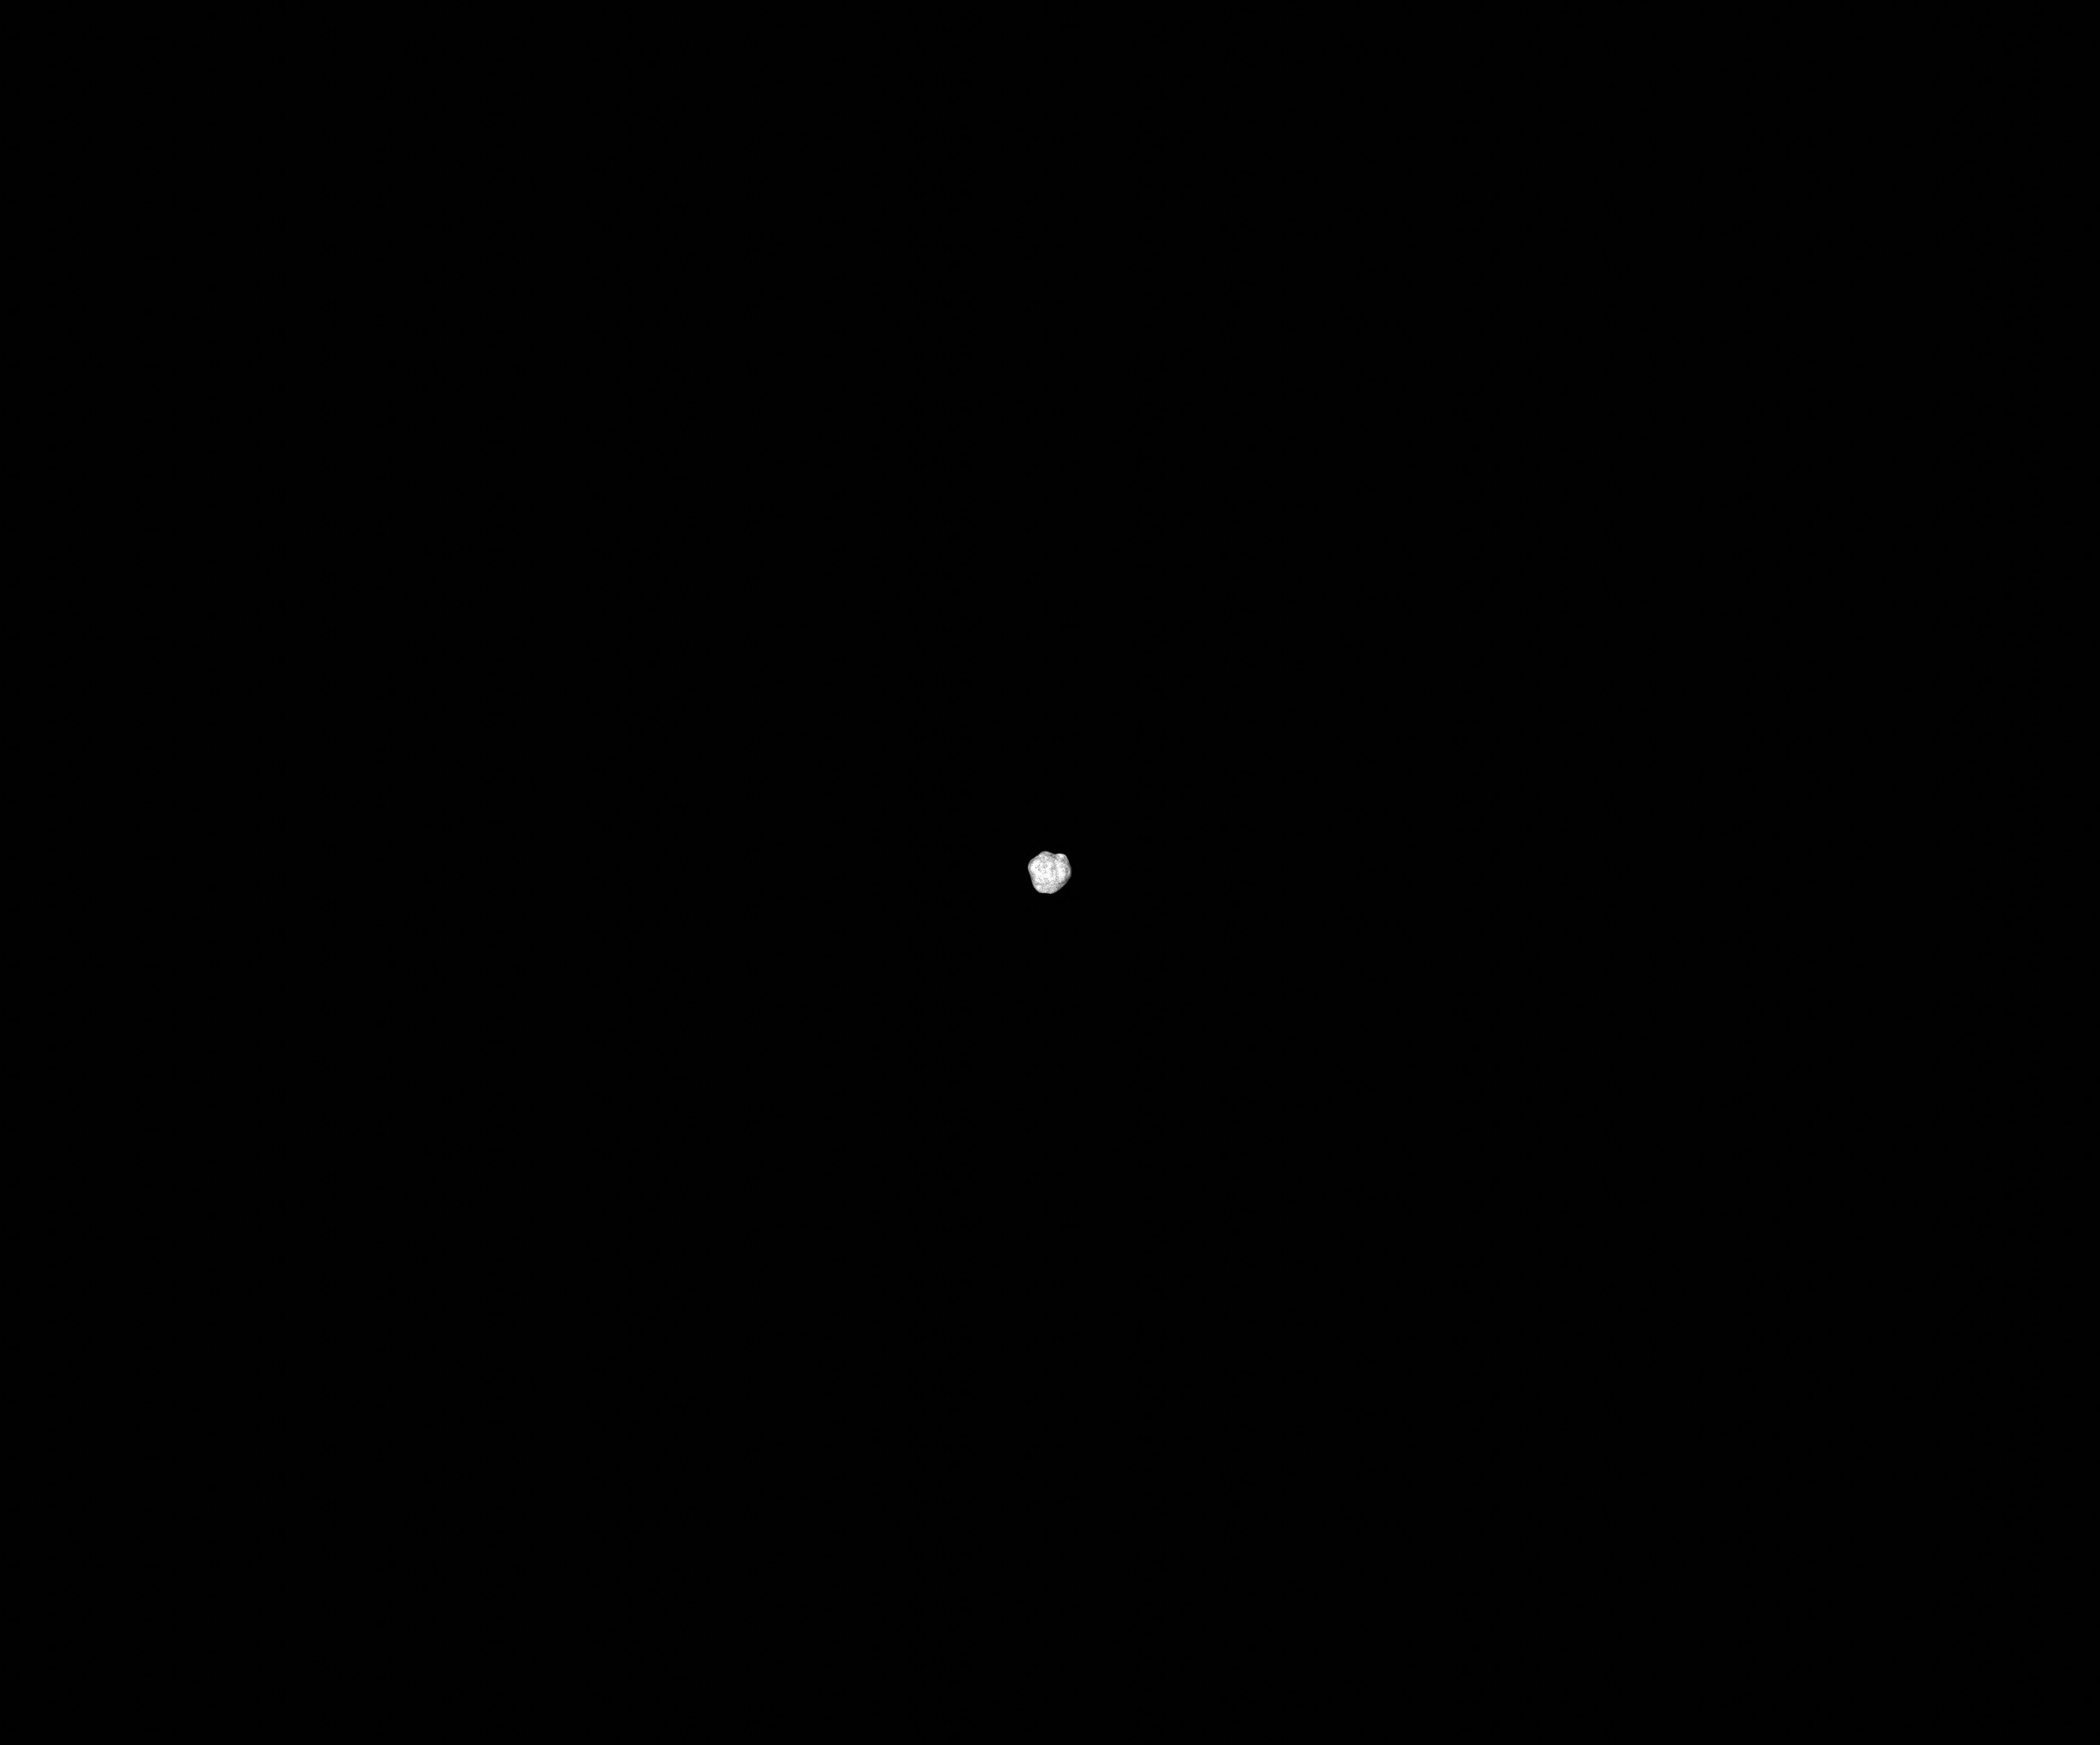
\includegraphics[height=8cm]{doc/thesis/0_figures/cv_skimage/SssbConstDist_2017-08-15T115851-679000.jpg}
    \end{center}
    \caption{SssbConstDist image used in benchmark.}
    \label{fig:bm_sssbconstdist}
\end{figure}

\section{OpenCV versus \gls{skimage} benchmark} \label{sec:app_cvskimage}

\begin{figure}[htb]
    \begin{center}
        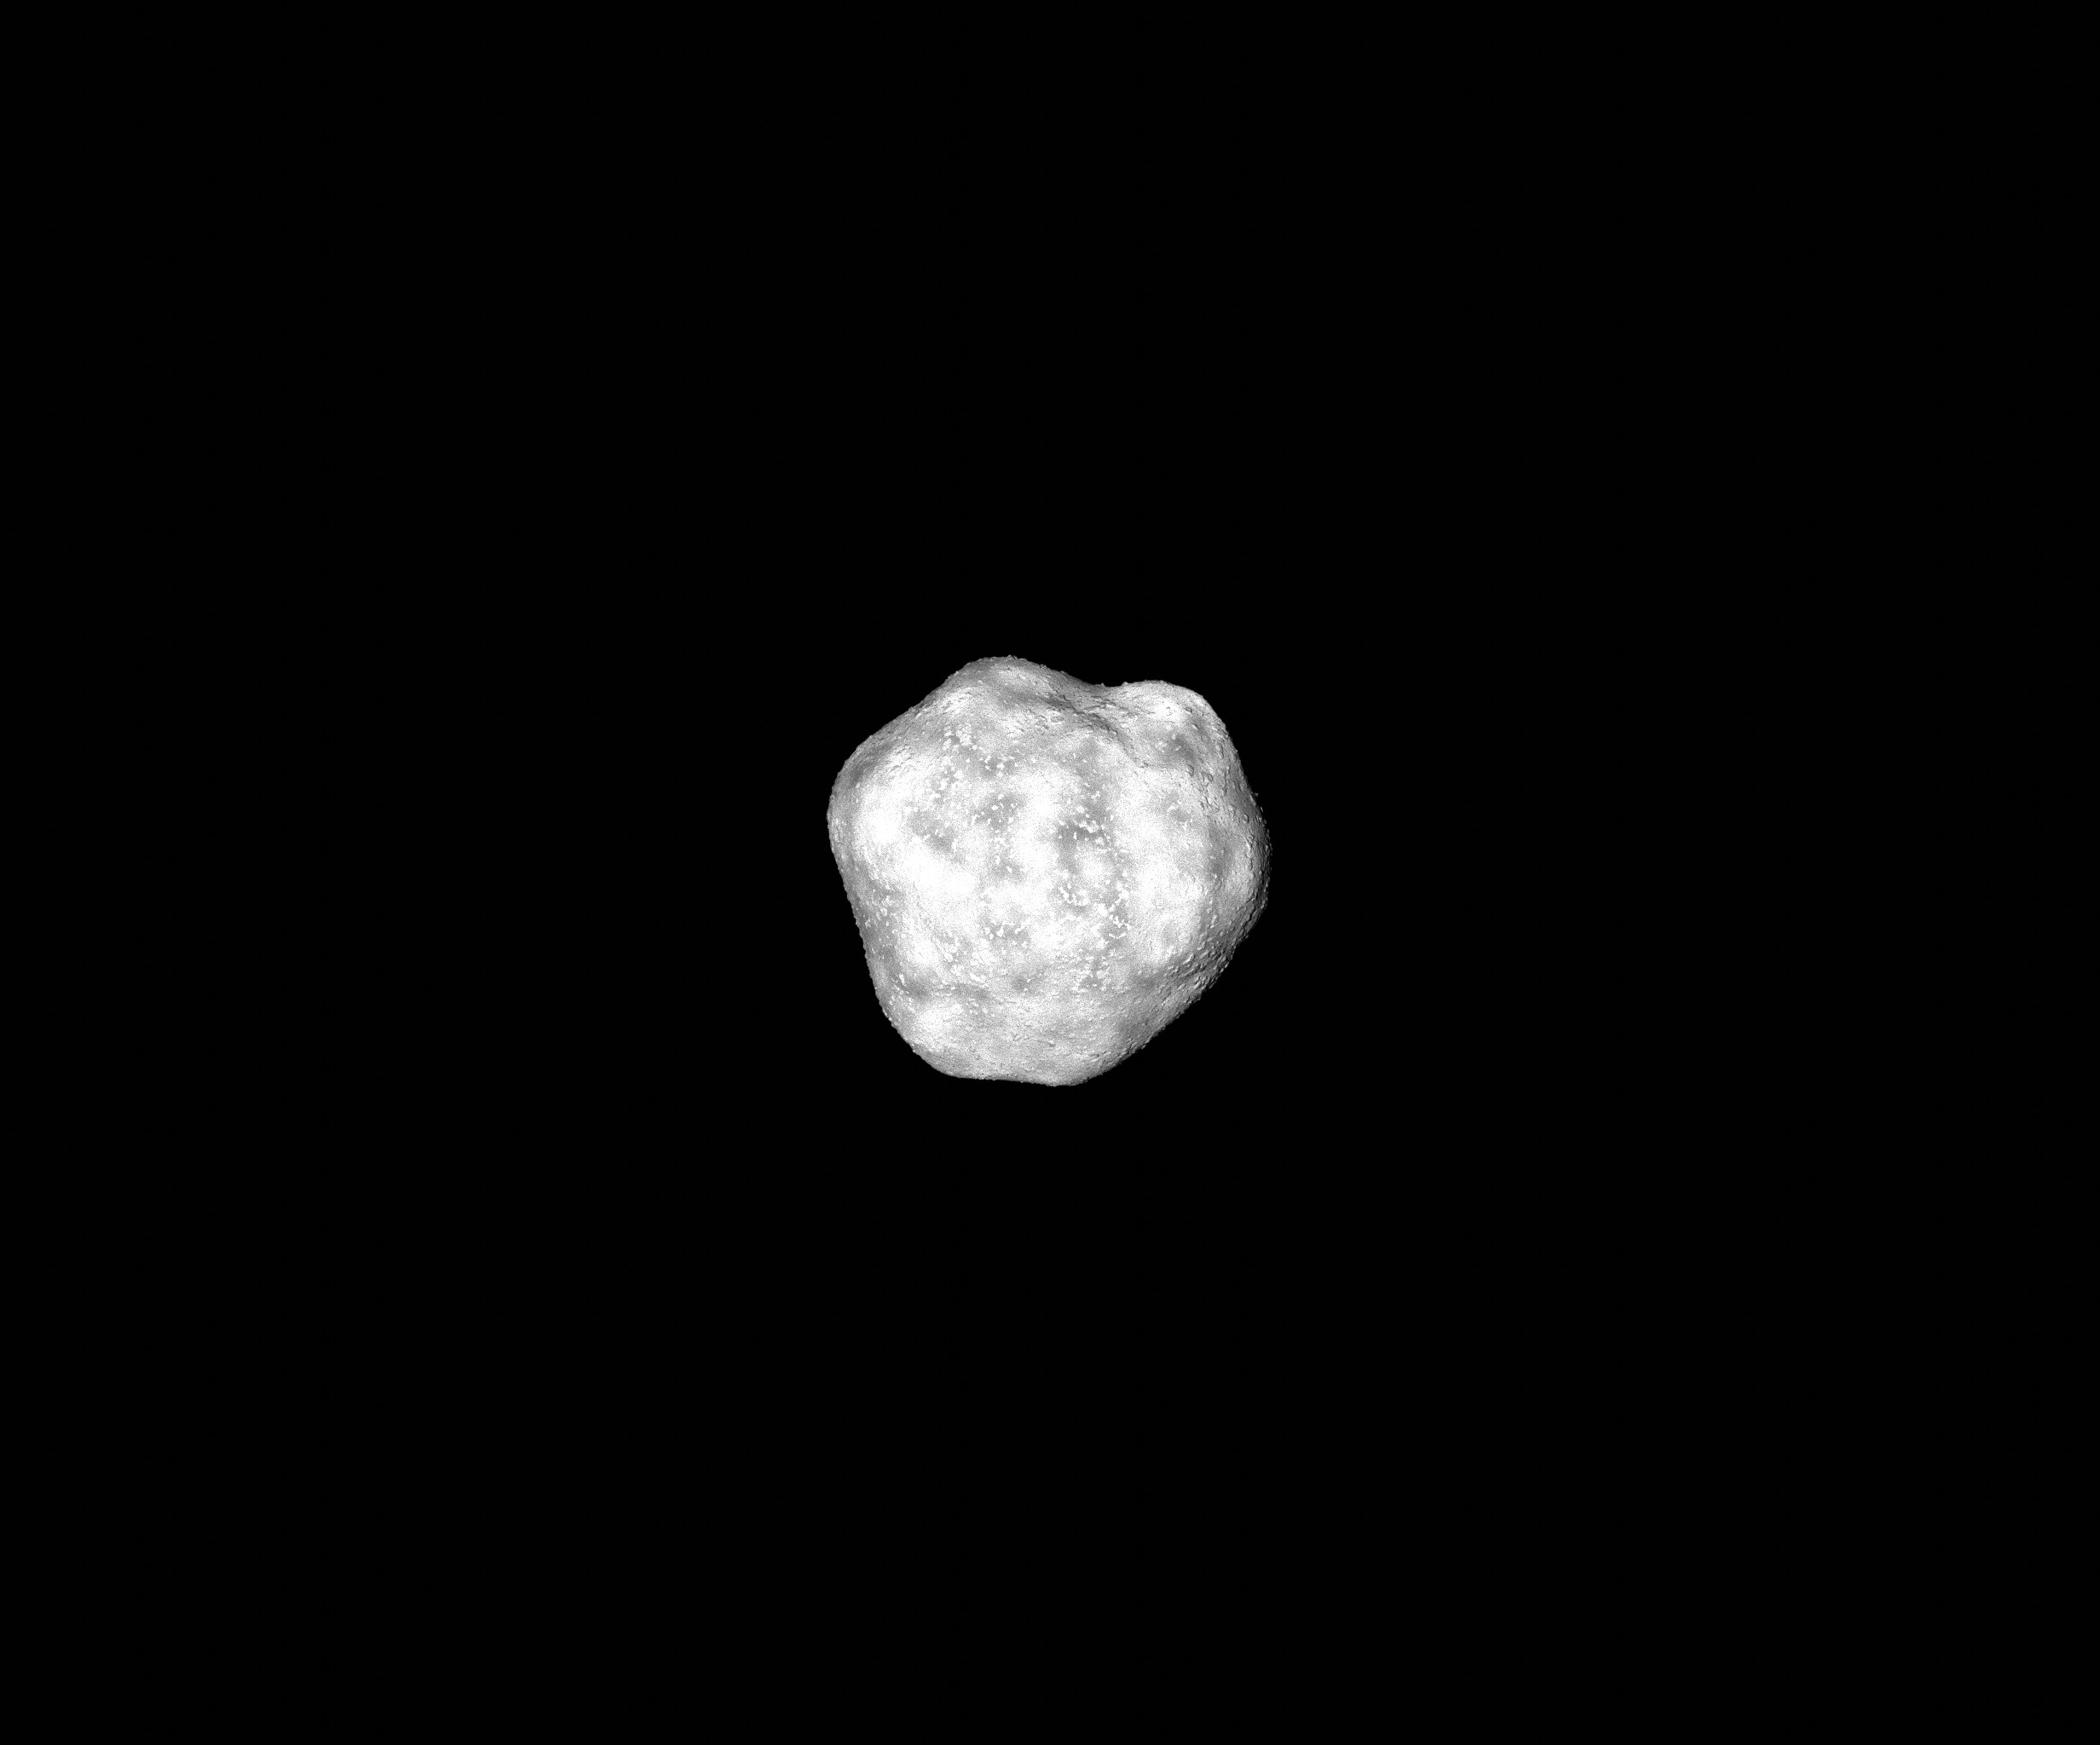
\includegraphics[height=8cm]{doc/thesis/0_figures/cv_skimage/SssbOnly_2017-08-15T115851-679000.jpg}
    \end{center}
    \caption{SssbOnly image used in benchmark.}
    \label{fig:bm_sssbonly}
\end{figure}

\begin{figure}[htb]
    \begin{center}
        
\includegraphics[height=8cm]{doc/thesis/0_figures/cv_skimage/Stars_2017-08-15T115841-334000.png}
    \end{center}
    \caption{Stars1 image used in benchmark. Based on 1804 stars of the UCAC4 catalog.}
    \label{fig:bm_stars1}
\end{figure}

\begin{figure}[htb]
    \begin{center}
        
\includegraphics[height=8cm]{doc/thesis/0_figures/cv_skimage/Stars_2017-08-15T115857-362000.png}
    \end{center}
    \caption{Stars2 image used in benchmark. Based on 51338 stars of the UCAC4 catalog.}
    \label{fig:bm_stars2}
\end{figure}

Figures \ref{fig:bm_light_ref} through \ref{fig:bm_stars2} are the images used in the benchmark. Their names are given in the respective caption.

\begin{figure}[htb]
    \begin{center}
        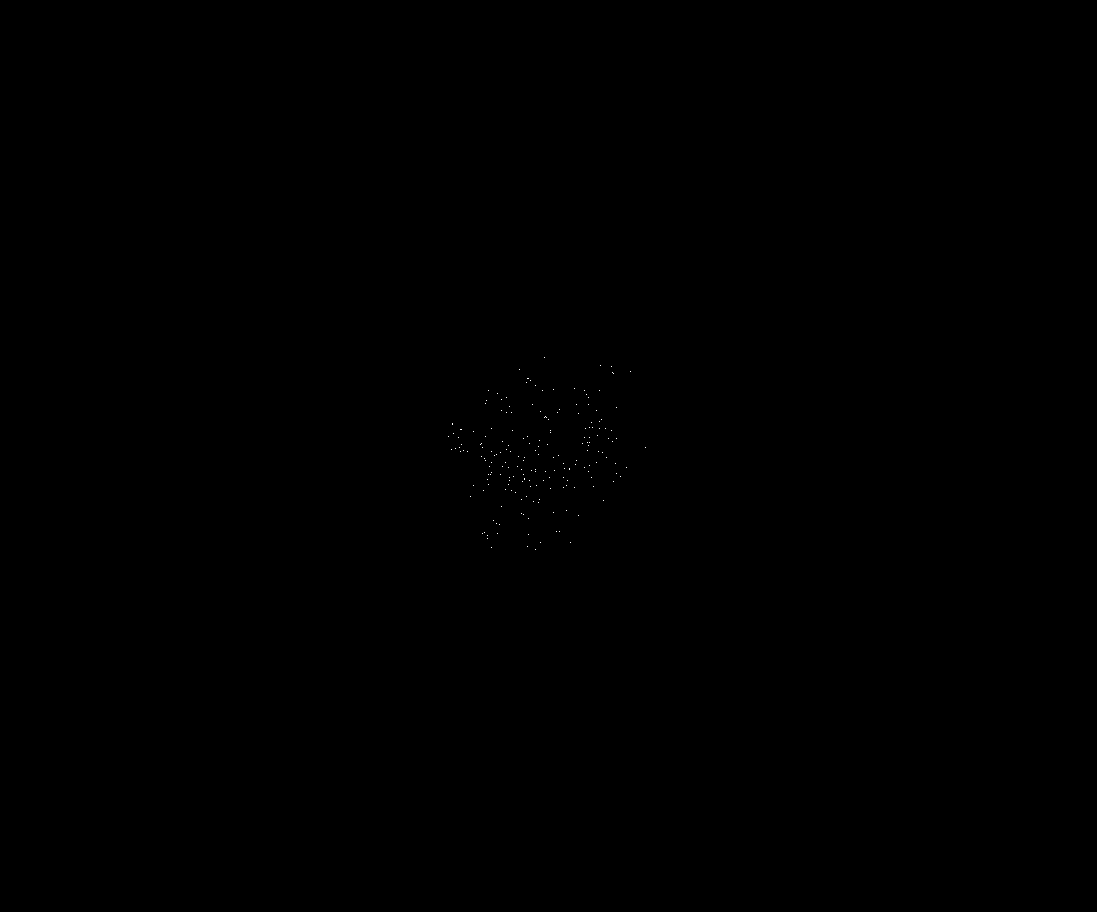
\includegraphics[height=8cm]{doc/thesis/0_figures/cv_skimage/diff_laptop.png}
    \end{center}
    \caption{Difference between \gls{skimage} and OpenCV Gaussian filtered SssbOnly image of the laptop.}
    \label{fig:bm_diff_laptop}
\end{figure}

\begin{figure}[htb]
    \begin{center}
        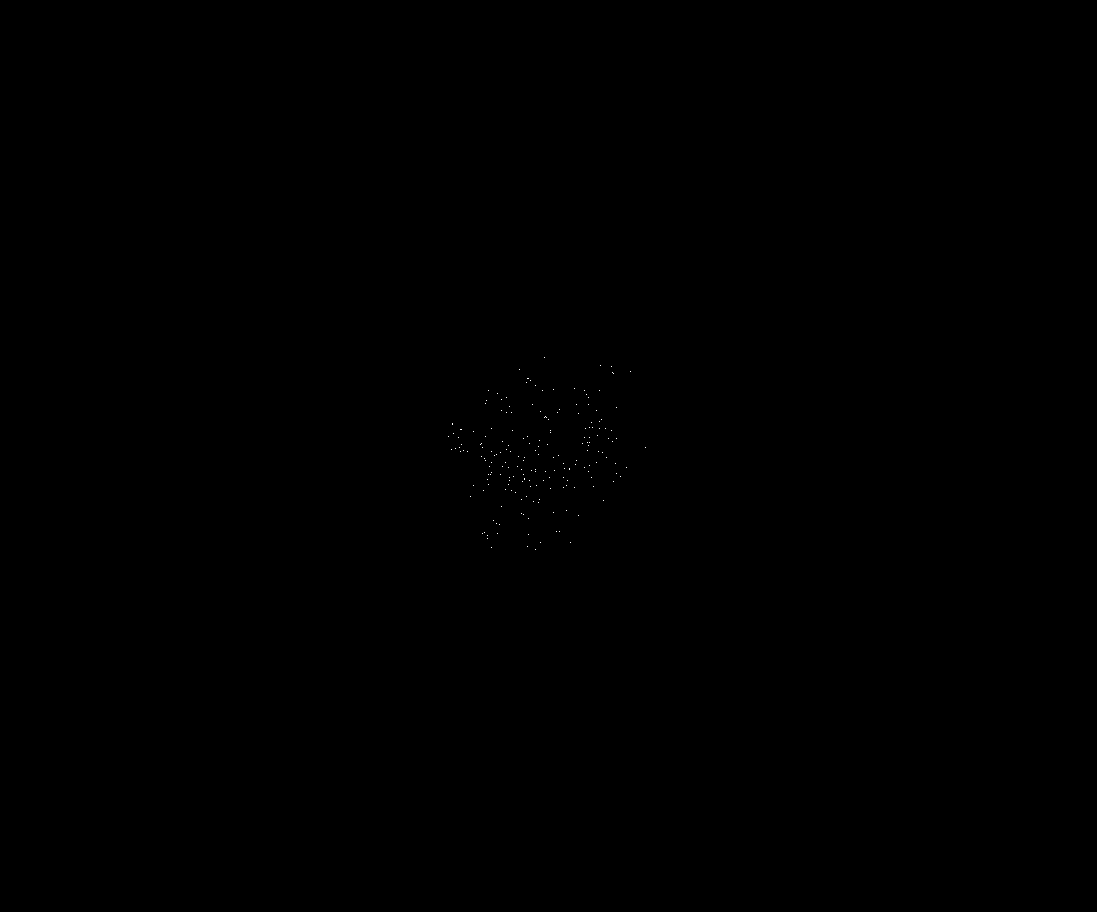
\includegraphics[height=8cm]{doc/thesis/0_figures/cv_skimage/diff_workstation.png}
    \end{center}
    \caption{Difference between \gls{skimage} and OpenCV Gaussian filtered SssbOnly image of the workstation.}
    \label{fig:bm_diff_workstation}
\end{figure}

Figures \ref{fig:bm_diff_laptop} and \ref{fig:bm_diff_workstation} show the difference of the SssbOnly image from the benchmark on the two different computers. Only a small fraction of pixels differ. As discussed previously, the maximum absolute difference is on the order of \SI{1e-6}{}, corresponding to the brightest point in each image. 